%%%%%
%file: pms.tex
%date: 21.3.2015
%author: Jan Wrona
%email: <xwrona00@stud.fit.vutbr.cz>
%project: Implementace algoritmu "Pipeline merge sort", PRL
%%%%%

\documentclass[a4paper, 12pt]{article}[21.3.2015]
  \usepackage[czech]{babel}
  \usepackage[utf8]{inputenc}
  \usepackage[T1]{fontenc}
  \usepackage[text={17cm, 24cm}, left=2cm, top=3cm]{geometry}

  \usepackage{amsmath}
  \usepackage{amsfonts}
  \usepackage{hyperref}
  \usepackage{graphicx}

  \graphicspath{ {./fig/} }

\begin{document}
%%%%
%%%%%
%file: title.tex
%date: 21.3.2015
%author: Jan Wrona
%email: <xwrona00@stud.fit.vutbr.cz>
%project: Implementace algoritmu pipeline merge sort, PRL
%%%%%

\begin{titlepage}
\begin{center}
\textsc{{\Huge Vysoké učení technické v Brně}\\
\medskip
{\huge Fakulta informačních technologií}}\\
\vspace{\stretch{0.382}}
{\LARGE Paralelní a distribuované algoritmy}\\
\medskip
{\Huge Implementace algoritmu pipeline merge sort}\\
\vspace{\stretch{0.618}}
\end{center}
{\Large \today \hfill Jan Wrona}
\end{titlepage}

%%%%

%%%%
\tableofcontents
%%%%

%%%%
\clearpage
\section{Úvod} \label{introduction}
%%%%
Cílem projektu je pomocí knihovny \emph{OpenMPI} implementovat v jazyce C/C++ algoritmus \emph{pipeline merge sort}. Vstupem programu je soubor \emph{numbers}, který obsahuje libovolná (tedy binární) data. Ta jsou programem interpretována jako čísla tak, že jeden bajt je chápán jako číslo v rozsahu \(<0-255>\). To jsou čísla určená k seřazení. Je požadováno tuto posloupnost vypsat na standardní výstup, čísla budou v vzájemně oddělena mezerou. Druhou částí předpokládaného výstupu je správně vzestupně seřazená vstupní posloupnost, čísla budou vzájemně oddělena novým řadkem.

%%%%
\section{Rozbor a analýza algoritmu} \label{analysis}
%%%%
Sekvenční verze algoritmu \emph{merge sort} pracuje se sekvencemi čísel. Vstupní posloupnost \(n\) čísel je rozdělena do \(n\) subsekvencí délky \(1\). Prvním průchodem je vytvořeno \(\frac{n}{2}\) seřazených subsekvencí délky \(2\), obecně je \(i\)-tým průchodem vytvořeno \(\frac{n}{2^i}\) seřazených subsekvencí délky \(2^i\). Každý průchod se skládá z \(n\) kroků a seřazení celé posloupnosti vyžaduje \(\log(n)\) průchodů. Celková časová složitost sekvenčního algoritmu merge sort je tak \(O(n\log(n))\).

Jedna z možností jak tento proces paralelizovat je pomocí pipelines, vzniká tak paralelní algoritmus pipeline merge sort. Tento algoritmus vyžaduje lineární pole procesorů délky \(\log(n) + 1\), kde \(n\) je délka vstupní posloupnosti čísel taková, že \(n = 2^r, r \in \mathbb{N}\). Procesory \(P_1\) až \(P_{r + 1}\) jsou rozděleny do tří skupin. První skupinu tvoří pouze procesor \(P_1\), který má na vstupu jednu pipeline obsahující vstupní posloupnost, ze které v každém kroku přečte jedno číslo a střídavě jej pošle na jednu ze svých dvou výstupních pipelines (vytváří tak subsekvence délky \(1\) pro procesor \(P_2\)). Druhou skupinu tvoří procesory \(P_2\) až \(P_r\), které přijímají na svých dvou vstupních pipelines subsekvence délky \(2^{i-2}\), kde \(i\) je číslo procesoru. Výstup této skupiny procesorů tvoří subsekvence, vytvořené sloučením dvou vstupních subsekvencí, které jsou postupně umisťovány do jedné z dvou výstupních pipelines. Třetí skupinu tvoří pouze procesor \(P_{r + 1}\). Ten zpracovává vstup stejně jako procesory předchozí skupiny, výstup v podobě seřazené vstupní posloupnosti však umisťuje do jediné pipeline. Procesory jsou pomocí dvou pipelines propojeny v pořadí, v jakém jsou očíslovány, tedy \(P_1\) předává subsekvence \(P_2\), \(P_2\) je předává \(P_3\) atd.

Při analýze časové složitosti se jeden výpočetní krok skládá z porovnání dvou čísel z vrcholů vstupních pipelines, vytažení většího/menšího z nich (v závisloti na vzestupném/sestupném řazení) a jeho umístění do výstupní pipeline. Z předchozího popisu lze vidět, že procesory nemohou pracovat vždy všechny současně, protože nemusí mít ve svých vstupních pipelines dostatek dat. Procesor \(P_1\) začíná pracovat okamžitě po startu, ostatní procesory až ve chvíli, kdy mají celou vstupní sekvenci v jedné z pipelines a jedno číslo z následující sekvence v druhé pipeline. Matematicky zapsáno, procesor \(P_1\) začíná pracovat v kroku 1. Krok, kterým začína procesor \(P_i\), je dán součtem délky sekvence plus 1 všech procesorů \(P_j, j \leq i\), tedy \(1 + \sum_{j = 0}^{i - 2}(2^{i - 2} + 1)\). Tato posloupnost lze zapsat jako \(2^n + n\), tento vztah je ale potřeba upravit s ohledem na číslování procesorů od jedničky následovně:
\[
	1 + \sum_{j = 0}^{i - 2}(2^{i - 2} + 1) = 2^{i - 1} + (i - 1).
\]
Obdobná situace je při ukončování výpočtu. Procesory svou práci končí spolu s poslední zpracovanou sekvencí, nikoliv všechny současně. V kroku, kdy procesor začal pracovat, bylo zpracováno jedno číslo. Zbývá jich tedy ještě \(n - 1\). Krok, kdy procesor ukončí svou práci, lze vyjádřit následovně:
\[
	2^{i - 1} + (i - 1) + (n - 1).
\]
Časová složitost je u paralelních algoritmů rovna času mezi startem výpočtu prvního procesoru a koncem výpočtu posledního procesoru. U zkoumaného algoritmu první procesor \(P_1\) začíná pracovat v čase 1 a poslední procesor \(P_{r + 1}\) končí výpočet v čase \(2^{r + 1 - 1} + (r + 1 - 1) + (n - 1) = 2^r + r + n - 1\). Z předpokladu, že \(n = 2^r\) můžeme odvodit \(r = \log(n)\) a po dosazení do předchozího výrazu vznikne \(2n + \log(n) - 1\). Časová složitor algoritmu je tedy lineání
\[
	O(2n + \log(n) - 1) = O(n).
\]

Cena je definována jako součin časové složitosti a počtu procesorů.
\[
	C(n) = O(n) * (\log(n) + 1) = O(n\log(n) + n) = O(n\log(n)).
\]
Nejrychlejší známé sekvenční řadící algoritmy dosahují časové složitosti \(O(n\log(n))\), cena pipeline merge sort je tedy optimální.

Paměťová složitost je dána potřebnou velikostí všech pipelines. Vstupní a výstupní pipelines mají velikost stejnou jako počet prvků řazené sekvence čísel \(n\). Každý procesor \(P_2\) až \(P_{r + 1}\) disponuje dvěma vstupními pipelines, každou o velikosti délky vstupní sekvence daného procesoru plus jedna, tedy \(2^{i - 2} + 1\). Celková paměťová složitost je tedy lineární
\[
	O(2n + \sum_{i = 2}^{\log(n) + 1}(2 * (2^{i - 2} + 1))) = O(4n + 2\log(n) - 2) = O(n).
\]
%%%%
\section{Komunikační protokol} \label{protocol}
%%%%
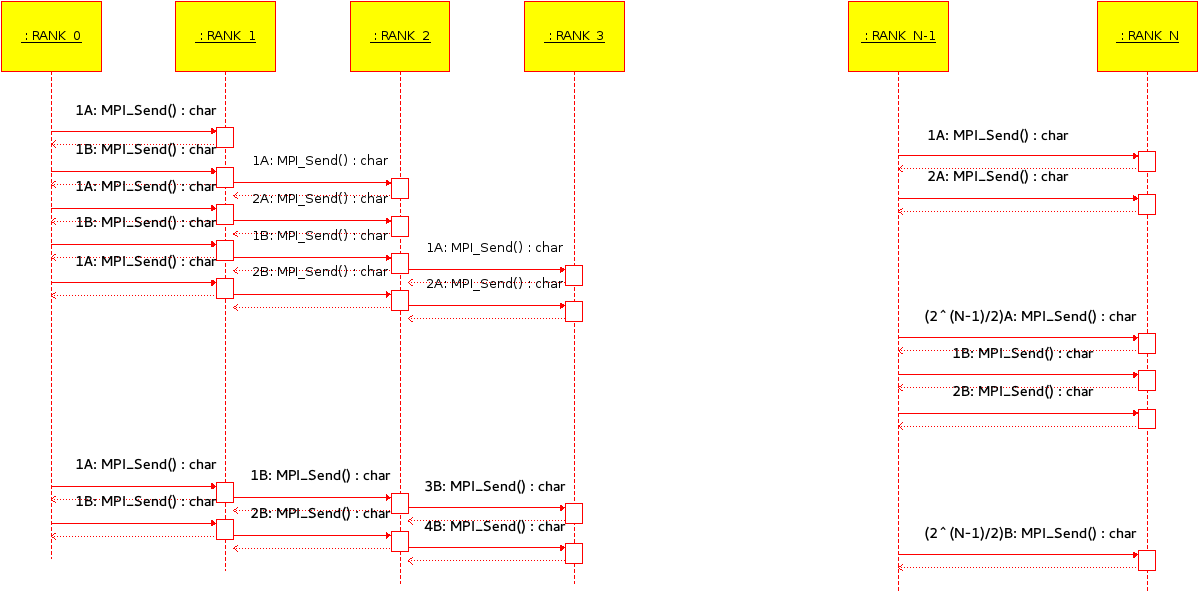
\includegraphics[width=\textwidth]{sequence_diagram}

%%%%
\section{Implementace, testování a experimenty} \label{experiments}
%%%%
Algoritmus jsem implementoval jak v jazce C s využitím vlastní implementace fronty, tak i v C++, kde byla použita \texttt{queue} z STL. Dvojí implementace jsem následně využil k sérii experimentů. Program v C byl mírně rychlejší, zároveň vlastní impelemtace fronty byla paměťově méně náročná (oboje pouze v řádu jednotek procent).

Ověření časové složitosti jsem prováděl měřením reálného času běhu části programu. Tato část obsahovala pouze reálné výpočetní jádro bez inicializací, výpisu do terminálu/souboru, atp. Začátek měření času byl spuštěn v jednom procesu po návratu z funkce \texttt{MPI\_Barrier()}, stejným způsobem bylo měření ukončeno, aby bylo zajištěno, že všechny procesory již ukončily svůj výpočet. Spolu s reálným časem probíhalo také měření spotřebovaného procesorového času všech procesorů, který byl následně sečten promocí \texttt{MPI\_Reduce()}.

Měření, jehož výsledky lze vidět na obrázku~\ref{complexity}, bylo provedeno na jediném výpočetním uzlu\footnote{ramdal.ics.muni.cz, \url{http://metavo.metacentrum.cz/pbsmon2/machine/ramdal.ics.muni.cz}}, na kterém byl alokován počet procesorů větší nebo roven počtu MPI procesorům. Tímto by měl být minimalizován vliv ostatních procesů a plánovače operačního systému, které mohou dobu běhu programu výrazně ovlivnit. Ze stejných důvodů bylo měření pro každou velikost vstupu opakováno pětkrát, z výsledných časů byl zaznamenán ten nejmenší.
\begin{figure}
	\centering
	\resizebox{\textwidth}{!}{% GNUPLOT: LaTeX picture with Postscript
\begingroup
  \makeatletter
  \providecommand\color[2][]{%
    \GenericError{(gnuplot) \space\space\space\@spaces}{%
      Package color not loaded in conjunction with
      terminal option `colourtext'%
    }{See the gnuplot documentation for explanation.%
    }{Either use 'blacktext' in gnuplot or load the package
      color.sty in LaTeX.}%
    \renewcommand\color[2][]{}%
  }%
  \providecommand\includegraphics[2][]{%
    \GenericError{(gnuplot) \space\space\space\@spaces}{%
      Package graphicx or graphics not loaded%
    }{See the gnuplot documentation for explanation.%
    }{The gnuplot epslatex terminal needs graphicx.sty or graphics.sty.}%
    \renewcommand\includegraphics[2][]{}%
  }%
  \providecommand\rotatebox[2]{#2}%
  \@ifundefined{ifGPcolor}{%
    \newif\ifGPcolor
    \GPcolortrue
  }{}%
  \@ifundefined{ifGPblacktext}{%
    \newif\ifGPblacktext
    \GPblacktexttrue
  }{}%
  % define a \g@addto@macro without @ in the name:
  \let\gplgaddtomacro\g@addto@macro
  % define empty templates for all commands taking text:
  \gdef\gplbacktext{}%
  \gdef\gplfronttext{}%
  \makeatother
  \ifGPblacktext
    % no textcolor at all
    \def\colorrgb#1{}%
    \def\colorgray#1{}%
  \else
    % gray or color?
    \ifGPcolor
      \def\colorrgb#1{\color[rgb]{#1}}%
      \def\colorgray#1{\color[gray]{#1}}%
      \expandafter\def\csname LTw\endcsname{\color{white}}%
      \expandafter\def\csname LTb\endcsname{\color{black}}%
      \expandafter\def\csname LTa\endcsname{\color{black}}%
      \expandafter\def\csname LT0\endcsname{\color[rgb]{1,0,0}}%
      \expandafter\def\csname LT1\endcsname{\color[rgb]{0,1,0}}%
      \expandafter\def\csname LT2\endcsname{\color[rgb]{0,0,1}}%
      \expandafter\def\csname LT3\endcsname{\color[rgb]{1,0,1}}%
      \expandafter\def\csname LT4\endcsname{\color[rgb]{0,1,1}}%
      \expandafter\def\csname LT5\endcsname{\color[rgb]{1,1,0}}%
      \expandafter\def\csname LT6\endcsname{\color[rgb]{0,0,0}}%
      \expandafter\def\csname LT7\endcsname{\color[rgb]{1,0.3,0}}%
      \expandafter\def\csname LT8\endcsname{\color[rgb]{0.5,0.5,0.5}}%
    \else
      % gray
      \def\colorrgb#1{\color{black}}%
      \def\colorgray#1{\color[gray]{#1}}%
      \expandafter\def\csname LTw\endcsname{\color{white}}%
      \expandafter\def\csname LTb\endcsname{\color{black}}%
      \expandafter\def\csname LTa\endcsname{\color{black}}%
      \expandafter\def\csname LT0\endcsname{\color{black}}%
      \expandafter\def\csname LT1\endcsname{\color{black}}%
      \expandafter\def\csname LT2\endcsname{\color{black}}%
      \expandafter\def\csname LT3\endcsname{\color{black}}%
      \expandafter\def\csname LT4\endcsname{\color{black}}%
      \expandafter\def\csname LT5\endcsname{\color{black}}%
      \expandafter\def\csname LT6\endcsname{\color{black}}%
      \expandafter\def\csname LT7\endcsname{\color{black}}%
      \expandafter\def\csname LT8\endcsname{\color{black}}%
    \fi
  \fi
  \setlength{\unitlength}{0.0500bp}%
  \begin{picture}(11338.00,5668.00)%
    \gplgaddtomacro\gplbacktext{%
      \csname LTb\endcsname%
      \put(1210,3538){\makebox(0,0)[r]{\strut{} 0}}%
      \put(1210,3804){\makebox(0,0)[r]{\strut{} 0.001}}%
      \put(1210,4071){\makebox(0,0)[r]{\strut{} 0.002}}%
      \put(1210,4337){\makebox(0,0)[r]{\strut{} 0.003}}%
      \put(1210,4604){\makebox(0,0)[r]{\strut{} 0.004}}%
      \put(1210,4870){\makebox(0,0)[r]{\strut{} 0.005}}%
      \put(1210,5137){\makebox(0,0)[r]{\strut{} 0.006}}%
      \put(1210,5403){\makebox(0,0)[r]{\strut{} 0.007}}%
      \put(1342,3318){\makebox(0,0){\strut{} 0}}%
      \put(2110,3318){\makebox(0,0){\strut{} 200}}%
      \put(2877,3318){\makebox(0,0){\strut{} 400}}%
      \put(3645,3318){\makebox(0,0){\strut{} 600}}%
      \put(4412,3318){\makebox(0,0){\strut{} 800}}%
      \put(5180,3318){\makebox(0,0){\strut{} 1000}}%
      \put(176,4470){\rotatebox{-270}{\makebox(0,0){\strut{}Čas [s]}}}%
      \put(3307,2988){\makebox(0,0){\strut{}Délka vstupní posloupnosti}}%
    }%
    \gplgaddtomacro\gplfronttext{%
      \csname LTb\endcsname%
      \put(4285,5230){\makebox(0,0)[r]{\strut{}walltime}}%
    }%
    \gplgaddtomacro\gplbacktext{%
      \csname LTb\endcsname%
      \put(6747,3538){\makebox(0,0)[r]{\strut{} 0}}%
      \put(6747,3849){\makebox(0,0)[r]{\strut{} 500}}%
      \put(6747,4160){\makebox(0,0)[r]{\strut{} 1000}}%
      \put(6747,4471){\makebox(0,0)[r]{\strut{} 1500}}%
      \put(6747,4781){\makebox(0,0)[r]{\strut{} 2000}}%
      \put(6747,5092){\makebox(0,0)[r]{\strut{} 2500}}%
      \put(6747,5403){\makebox(0,0)[r]{\strut{} 3000}}%
      \put(6879,3318){\makebox(0,0){\strut{} 0}}%
      \put(7556,3318){\makebox(0,0){\strut{} 1e+08}}%
      \put(8233,3318){\makebox(0,0){\strut{} 2e+08}}%
      \put(8910,3318){\makebox(0,0){\strut{} 3e+08}}%
      \put(9587,3318){\makebox(0,0){\strut{} 4e+08}}%
      \put(10264,3318){\makebox(0,0){\strut{} 5e+08}}%
      \put(10941,3318){\makebox(0,0){\strut{} 6e+08}}%
      \put(5845,4470){\rotatebox{-270}{\makebox(0,0){\strut{}Čas [s]}}}%
      \put(8910,2988){\makebox(0,0){\strut{}Délka vstupní posloupnosti}}%
    }%
    \gplgaddtomacro\gplfronttext{%
      \csname LTb\endcsname%
      \put(9954,5230){\makebox(0,0)[r]{\strut{}walltime}}%
    }%
    \gplgaddtomacro\gplbacktext{%
      \csname LTb\endcsname%
      \put(1210,704){\makebox(0,0)[r]{\strut{} 0}}%
      \put(1210,874){\makebox(0,0)[r]{\strut{} 0.005}}%
      \put(1210,1043){\makebox(0,0)[r]{\strut{} 0.01}}%
      \put(1210,1213){\makebox(0,0)[r]{\strut{} 0.015}}%
      \put(1210,1383){\makebox(0,0)[r]{\strut{} 0.02}}%
      \put(1210,1552){\makebox(0,0)[r]{\strut{} 0.025}}%
      \put(1210,1722){\makebox(0,0)[r]{\strut{} 0.03}}%
      \put(1210,1891){\makebox(0,0)[r]{\strut{} 0.035}}%
      \put(1210,2061){\makebox(0,0)[r]{\strut{} 0.04}}%
      \put(1210,2231){\makebox(0,0)[r]{\strut{} 0.045}}%
      \put(1210,2400){\makebox(0,0)[r]{\strut{} 0.05}}%
      \put(1210,2570){\makebox(0,0)[r]{\strut{} 0.055}}%
      \put(1342,484){\makebox(0,0){\strut{} 0}}%
      \put(2110,484){\makebox(0,0){\strut{} 200}}%
      \put(2877,484){\makebox(0,0){\strut{} 400}}%
      \put(3645,484){\makebox(0,0){\strut{} 600}}%
      \put(4412,484){\makebox(0,0){\strut{} 800}}%
      \put(5180,484){\makebox(0,0){\strut{} 1000}}%
      \put(176,1637){\rotatebox{-270}{\makebox(0,0){\strut{}Čas [s]}}}%
      \put(3307,154){\makebox(0,0){\strut{}Délka vstupní posloupnosti}}%
    }%
    \gplgaddtomacro\gplfronttext{%
      \csname LTb\endcsname%
      \put(4285,2397){\makebox(0,0)[r]{\strut{}cputime}}%
    }%
    \gplgaddtomacro\gplbacktext{%
      \csname LTb\endcsname%
      \put(6879,704){\makebox(0,0)[r]{\strut{} 0}}%
      \put(6879,971){\makebox(0,0)[r]{\strut{} 10000}}%
      \put(6879,1237){\makebox(0,0)[r]{\strut{} 20000}}%
      \put(6879,1504){\makebox(0,0)[r]{\strut{} 30000}}%
      \put(6879,1770){\makebox(0,0)[r]{\strut{} 40000}}%
      \put(6879,2037){\makebox(0,0)[r]{\strut{} 50000}}%
      \put(6879,2303){\makebox(0,0)[r]{\strut{} 60000}}%
      \put(6879,2570){\makebox(0,0)[r]{\strut{} 70000}}%
      \put(7011,484){\makebox(0,0){\strut{} 0}}%
      \put(7666,484){\makebox(0,0){\strut{} 1e+08}}%
      \put(8321,484){\makebox(0,0){\strut{} 2e+08}}%
      \put(8976,484){\makebox(0,0){\strut{} 3e+08}}%
      \put(9631,484){\makebox(0,0){\strut{} 4e+08}}%
      \put(10286,484){\makebox(0,0){\strut{} 5e+08}}%
      \put(10941,484){\makebox(0,0){\strut{} 6e+08}}%
      \put(5845,1637){\rotatebox{-270}{\makebox(0,0){\strut{}Čas [s]}}}%
      \put(8976,154){\makebox(0,0){\strut{}Délka vstupní posloupnosti}}%
    }%
    \gplgaddtomacro\gplfronttext{%
      \csname LTb\endcsname%
      \put(9954,2397){\makebox(0,0)[r]{\strut{}cputime}}%
    }%
    \gplbacktext
    \put(0,0){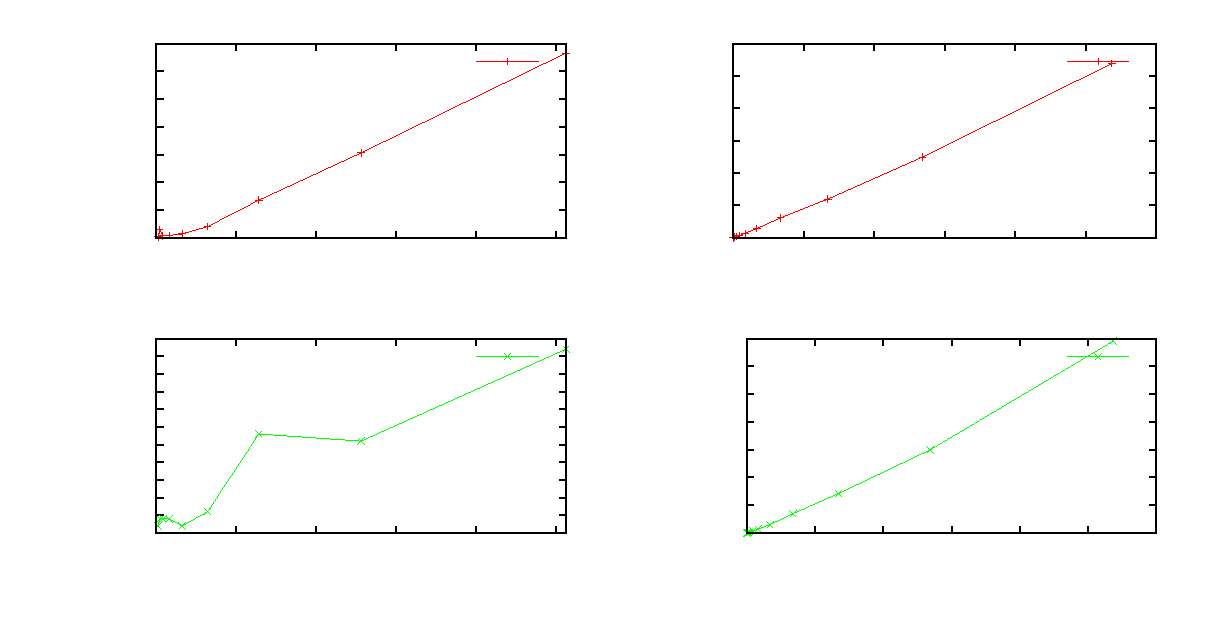
\includegraphics{fig/complexity}}%
    \gplfronttext
  \end{picture}%
\endgroup
} %! keeps aspect ratio
	\caption{Výsledky měření časové složitosti. Reálný čas nahoře, procesorový čas dole.}
	\label{complexity}
\end{figure}

%%%%
\section{Závěr}\label{conclusion}
%%%%
Rozbor algoritmu v sekci~\ref{analysis} ukazuje, že teoretická časová i paměťová složitost algoritmu je lineární, což při použití daného počtu procesorů dělá algoritmus také optimálním. Ve stejné sekci je také popsána vzájemná komunikace procesorů a v kapitole~\ref{protocol} je tento princip znázorněn pomocí sekvenčního diagramu. Po implementaci algoritmu byla provedena řada testů a experimentů, které si kladly za cíl ověřit teoretickou časovou složitost. Jak lze vidět v sekci~\ref{experiments}, naměřené časy pro různé délky vstupních posloupností odpovídají lineárnímu průběhu a teoretickou složitos tak potvrzují i prakticky.

\end{document}
